\section{Tietorakenteen arviointi}\label{tulokset}

Luvussa \ref{mun} esitettiin sisäkkäispistepuun solmujen sisältämien ruudukoiden mahdollistama yksinkertainen kompressiotekniikka ja algoritmeja puun rakentamiseen ja visualisointiin. Ensin mitataan sisäkkäispistepuun rakentamisen, tallentamisen ja läpikäynnin suorituskykyä ja arvioidaan kompression vaikutusta siihen. Tämän jälkeen mitataan pistepilvien visualisointinopeutta eri tekniikoilla käyttäen maiseman läpi kulkevia kamera-ajoja. Testikoneessa on Intel i7-8850H -suoritin, 32 gigatavua keskusmuistia, SSD-levy ja Nvidia Quadro P2000 -näytönohjain.  

Tietorakenteen rakentamista, tallentamista ja muistiin lataamista arvioitiin kolmella pistepilvellä. \emph{Konehuone}-pilvi sisälsi 20 keilausta, jotka veivät 18,7 gigatavua tilaa tallennettuna pakkaamattomaan tekstitiedostoon. Keilauksista muodostettiin puu, jossa oli 546 572 600 pistettä 528 017:ssa solmussa, jotka jakautuivat yhdeksälle tasolle. \emph{Toimisto} sisälsi 8,43 gigatavua pisteitä 21 keilauksesta ja siitä muodostetussa puussa oli 240 727 221 pistettä 608 002:ssa solmussa 11:llä tasolla. \emph{Pumput} oli testattavista pienin, vain 41:n megatavun kokoinen pistepilvi. Siinä oli 5 keilausta, joista rakennetussa puussa oli 1 213 990 pistettä 4561:ssä solmussa seitsemällä tasolla.  

\begin{table}[h]
    \begin{tabular}{|l|l|l|l|}
    \hline
    \textbf{pisteiden esitysmuoto} & \textbf{tiedoston koko} & \textbf{rakentaminen ja tallentaminen} & \textbf{läpikäynti} \\ \hline
    16 tavua       & 8,17GB             & 2574s = 42min 54s              & 6227ms     \\
    8 tavua        & 4,10GB             & 1652s = 27min 32s             & 16190ms    \\
    4 tavua        & 2,07GB             & 1602s = 26min 42s             & 13462ms    \\ \hline
    \end{tabular}
    \caption{Konehuone-pilvestä muodostetun oktettipuun rakentaminen ja pisteiden läpikäyminen}
    \label{taulukko:konehuone}
\end{table}


\begin{table}[h]
    \begin{tabular}{|l|l|l|l|}
    \hline
    \textbf{pisteiden esitysmuoto} & \textbf{tiedoston koko} & \textbf{rakentaminen ja tallentaminen} & \textbf{läpikäynti} \\ \hline
    16 tavua & 3,59GB              & 891s = 14min 51s              & 2763ms     \\
    8 tavua  & 1,83GB              & 724s = 12min 4s               & 8492ms     \\
    4 tavua & 961MB               & 712s = 11min 52s              & 6985ms     \\ \hline
    \end{tabular}
    \caption{Toimisto-pilvestä muodostetun oktettipuun rakentaminen ja pisteiden läpikäyminen}
    \label{taulukko:toimisto}
\end{table}

\begin{table}[h]
    \begin{tabular}{|l|l|l|l|}
    \hline
    \textbf{pisteiden esitysmuoto} & \textbf{tiedoston koko} & \textbf{rakentaminen ja tallentaminen} & \textbf{läpikäynti} \\ \hline
    16 tavua       & 18,6MB              & 12s                           & 14ms       \\ \hline
    8 tavua      & 9,57MB              & 10s                           & 36ms       \\ \hline
    4 tavua      & 4,94MB              & 9s                            & 29ms       \\ \hline
    \end{tabular}
    \caption{Pumput-pilvestä muodostetun oktettipuun rakentaminen ja pisteiden läpikäyminen}
    \label{taulukko:pumput}
\end{table}

Taulukoissa \ref{taulukko:konehuone}, \ref{taulukko:toimisto} ja \ref{taulukko:pumput} on mitattu testipilvien rakentamiseen, tallentamiseen ja pisteiden läpikäyntiin kuluva aika ja binääritiedoston koko käyttäen kolmea luvussa \ref{kompressio} käytettyä pisteiden esitysmuotoa: maailmakoordinaatit ja väri (16 tavua), ruudukon solun indeksi ja väri (8 tavua), sekä solun suhteelliset koordinaatit ja laserkeilaimeen takaisin heijastuneen valon intensiteetti (4 tavua). 

Yllätyksettömästi 16:n tavun pistedatan muistiin lataaminen ja läpikäyminen oli huomattavasti nopeampaa kuin kompressoitujen pisteiden. Nelitavuisten pisteiden lataaminen ja kompression purkaminen oli nopeampaa kuin kahdeksantavuisten. Tietorakennetta rakennettaessa näyttää siltä, että pistedatan kirjoittaminen levylle vie huomattavan osan suoritusajasta. Tästä syystä on ajansäästön kannalta kannattavaa käyttää laskenta-aikaa pistedatan kompressointiin, jotta kirjoitettavia tavuja olisi vähemmän. 

Tietorakenteen visualisointia arvioitaessa käytetään kahta pistepilveä. \emph{Ilmanvaihtohuone} on keilattu Elomatic Oy:n Jyväskylän toimiston ilmanvaihdon konehuoneesta ja siinä on 13 keilausta, joista muodostetussa puussa on 506 366 789 pistettä 267 641 solmussa kahdeksassa tasossa. \emph{Worksite}-pilvi on Leica Geosystemsin testidataa, joka sisältää 7 keilausta, joiden 53 881 180 pistettä jakautuu 543 105 solmuun yhdeksälle puun tasolle. 

\begin{figure}[h]
    \centering
    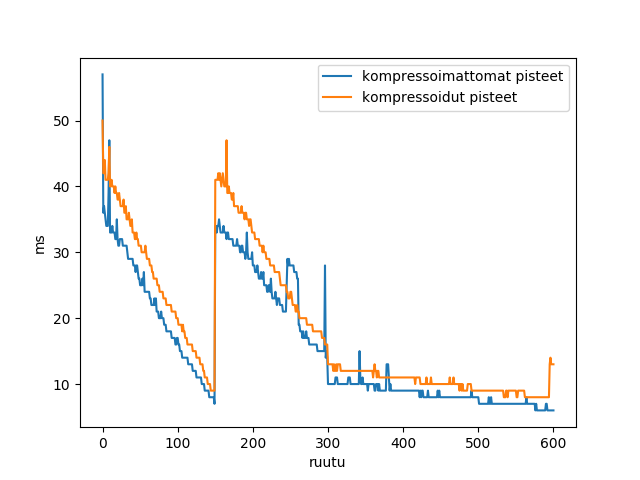
\includegraphics[width=0.9\textwidth]{tuloksia/worksite_compressed_vs_uncompressed.png}
    \caption{Worksite-pilven kahden miljoonan pisteen piirtämiseen vaadittu aika millisekunteina käyttäen kompressoimattomia 16:n tavun pisteitä ja kahdeksaan tavuun kompressoituja pisteitä.}
    \label{ws_compr}
\end{figure}

Arvioidaan ensin luvussa \ref{kompressio} esitellyn kompression vaikutusta pistepilven visualisointiaikaan. Kuvassa \ref{ws_compr} on esitetty kaavio kahden miljoonan pisteen piirtämisen vaatimasta ajasta kamera-ajon jokaisella ruudunpäivityksellä. Sininen viiva kuvaa piirtoaikaa kompressoimattomilla pisteillä ja oranssi viiva värit säilyttävällä kompressiolla. Visualisoinnissa on käytetty luvussa \ref{render} esiteltyä puskurivirta-algoritmia. 

Kamera-ajo alkaa maiseman reunalta ja kulkee työmaan ohi lähestyen sen reunaa siten, että näkyvissä olevien puun solmujen määrä laskee tasaisesti. Tämä näkyy myös kuvassa \ref{ws_compr} ruudun visualisointiajan laskiessa. Näkymäkarton sisällä olevien solmujen määrä kasvaa äkkinäisesti noin 150:nnen ruudun kohdalla, kun kamera kääntyy niin, että koko pilvi on näkyvissä. Lopuksi kamera lähestyy vastakkaista seinää ja näkyvissä olevien solmujen määrä laskee. 

Kuvaajasta huomataan, että kompressoimattomien 16-tavuisten pisteiden piirtäminen on jonkin verran nopeampaa kuin kompressoitujen kahdeksantavuisten pisteiden. Eron selittää kompression avaamiseen vaadittu laskenta. Jokaisesta kompressoidusta pisteestä etsitään kompressoidun pisteen indeksiä vastaava ruudukon solu ja lasketaan sen keskipiste. Visualisointiajan ero on kuitenkin pieni ja voidaan katsoa, että miltei puolittunut tallennustilan tarve oikeuttaa pistedatan kompression.

\begin{figure}[h] 
    \centering
    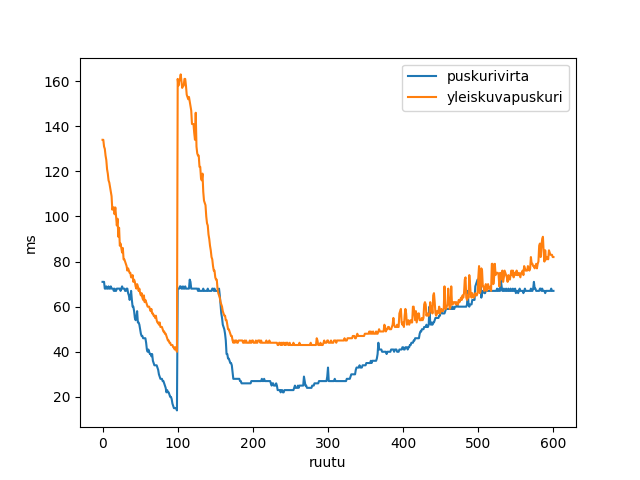
\includegraphics[width=0.9\textwidth]{tuloksia/ilmanvaihtohuone_ms_per_frame.png}
    \caption{Ilmanvaihtohuone: kahden miljoonan pisteen piirtämiseen vaadittu aika millisekunteina kahdella eri visualisointialgoritmilla.}
    \label{iv_ms}
\end{figure}

Luvussa \ref{render} esiteltiin puskurivirran lisäksi yleiskuvapuskuria käyttävä algoritmi, joka pitää osaa pistepilvestä näytönohjaimen muistissa. Kuvassa \ref{iv_ms} on mitattu kahden miljoonan pisteen piirtoaikaa ilmanvaihtohuone-pilvessä. Sininen viiva kuvaa piirtoaikaa käytettäessä pelkkää puskurivirtaa ja oranssin viivan kuvaamassa mittauksessa on ensin visualisoitu yleiskuvapuskuri, minkä jälkeen jäljelle jäävät puun solmut on järjestetty kuvaruudulle projisoidun koon mukaan ja piirretty puskurivirralla. Yleiskuvapuskurissa on puun neljä ensimmäistä tasoa, joissa on yhteensä 286 solmua ja niissä 723 834 pistettä.

Ilmanvaihtohuoneen kamera-ajo alkaa huoneen reunalta kameran osoittaessa vastakkaiselle seinälle. Kamera liikkuu kohti seinää, jolloin visualisoitavien solmujen määrä vähenee. Kameran saavutettua vastakkaisen seinän noin sadan ruudun jälkeen se kääntyy ympäri osoittamaan huoneen poikki. Näkyvissä olevien solmujen äkkinäinen kasvaminen näkyy jyrkkänä piikkinä kuvassa \ref{iv_ms}. Tämän jälkeen kamera lähestyy taas seinää ja piirtoaika vähenee. Lopuksi kamera peruuttaa pois päin seinästä ja näkyvillä olevien solmujen kasvava määrä pitkittää ruutujen visualisointia.

\begin{figure}[h]
    \centering
    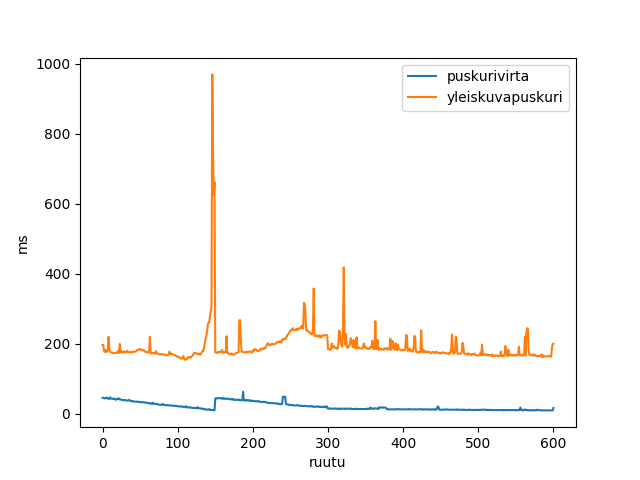
\includegraphics[width=0.9\textwidth]{tuloksia/worksite_ms_per_frame.png}
    \caption{Worksite-pilven kahden miljoonan pisteen piirtämiseen vaadittu aika millisekunteina kahdella eri visualisointialgoritmilla}
    \label{ws_ms}
\end{figure}

Kuvassa \ref{ws_ms} on tehty vastaavat mittaukset worksite-pilvelle. Oranssin viivan kuvaamassa visualisointitavassa on yleiskuvapuskurissa puun viisi ylintä kerrosta, 1862 solmua ja 481 663 pistettä.

\begin{figure}
    \subfloat[]{
        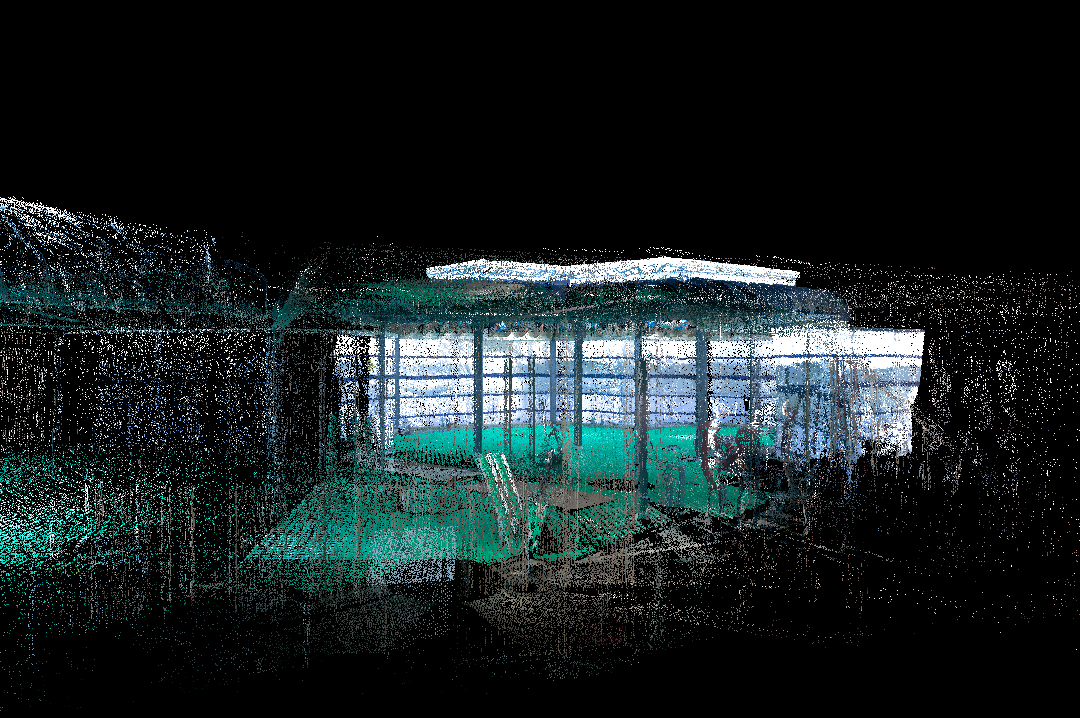
\includegraphics[width=.5\linewidth]{tuloksia/worksite_2M/worksite_stream.png}
    }
    \subfloat[]{
        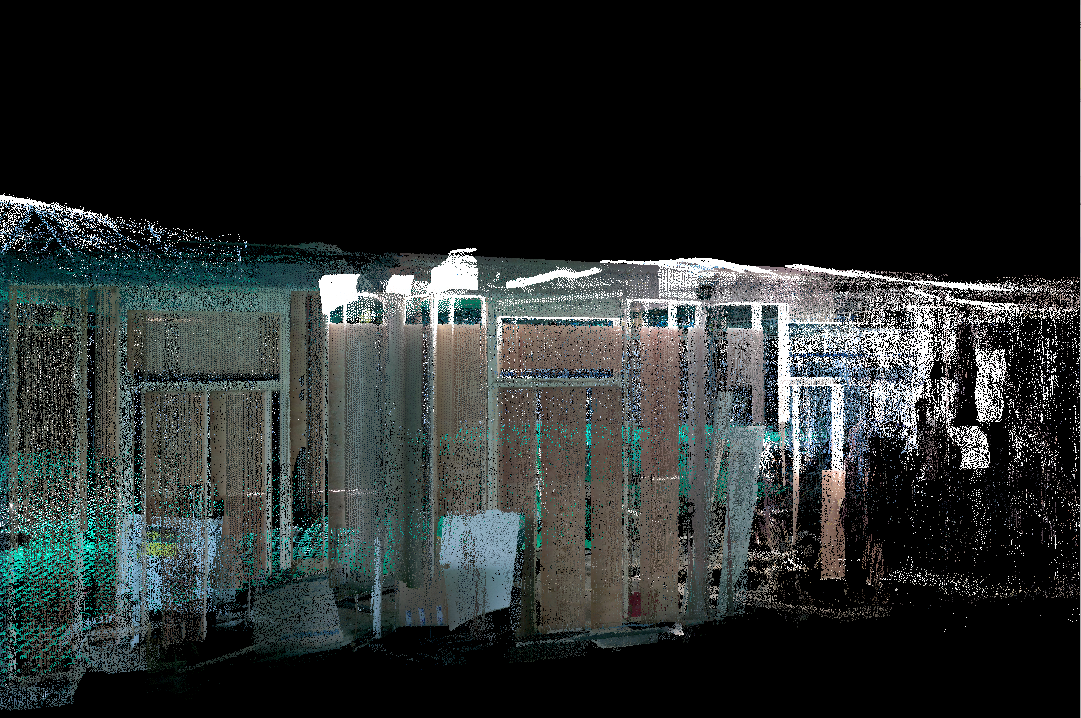
\includegraphics[width=.5\linewidth]{tuloksia/worksite_2M/worksite_overviewbuf.png}
    }
    \caption{Worksite-pilvi visualisoitu kahdella miljoonalla pisteellä käyttäen (a) pelkkää puskurivirtaa ja (b) yleiskuvapuskurin ja puskurivirran yhdistelmällä. Oikeanpuoleisessa kuvassa oktettipuun solmujen järjestämisen ansiosta kameraa lähellä oleva seinä on piirretty korkeammalla pistetiheydellä kuin vasemmassa kuvassa. Pistepilvi on Leica Geosystemsin omaisuutta.}
    \label{img:worksite_vertailu}
\end{figure}

Mittauksista selviää, että pelkän puskurivirran käyttäminen puun visualisoinnissa on selkeästi nopeampaa kuin yleiskuvapuskurin ja puskurivirran yhdistelmällä. Tämä ero selittyy puun solmujen järjestämiseen vaaditulla ajalla. Vaikka järjestäminen vie arvokasta laskenta-aikaa, voidaan sen katsoa parantavan lopputuloksen laatua. Kuvassa \ref{img:worksite_vertailu} vasemmalla puolella näkyy, kuinka puskurivirta on piirtänyt koko näkyvillä olevan pistepilven samalla pistetiheydellä ja taaimmainen seinä näyttää tarkemmalta kuin kameraa lähempänä oleva. Oikeanpuoleisessa kuvassa puun solmut on yleiskuvan piirtämisen jälkeen järjestetty ruudulle projisoidun koon mukaan, minkä seurauksena etualalla oleva seinä näkyy selvästi.

\begin{figure}[h]
    \centering
    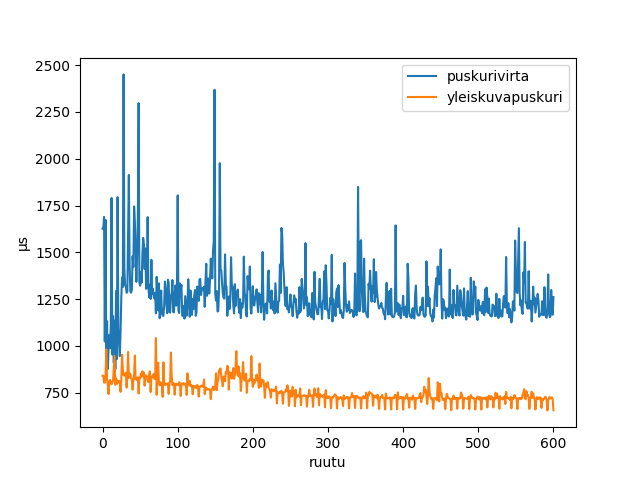
\includegraphics[width=0.9\textwidth]{tuloksia/worksite_overview.png}
    \caption{Worksite-pilvestä muodostetun puun viiden ylimmän tason visualisointiin käytetty aika mikrosekunteina puskurivirralla ja kun pisteet ovat valmiiksi yleiskuvapuskurissa näytönohjaimen muistissa.}
    \label{ws_ovw}
\end{figure}

Kameran liikkuessa pistepilven ohi riittää usein piirtää vain karkea yleiskuva pilvestä. Kun yleiskuvan pisteet pidetään näytönohjaimen muistissa, on niiden piirtäminen jokaisella ruudunpäivityksellä nopeaa. Kuvassa \ref{ws_ovw} on verrattu yleiskuvan piirtämistä kun yleiskuvapuskuri on valmiiksi näytönohjaimen muistissa siihen, kun pisteet ladataan keskusmuistista puskurivirralla näytönohjaimelle. Yleiskuvapuskurin tapauksessa piirtoaika on mitattu piirtokomennon suorittamisesta siihen, että näytönohjain on saanut kaikki pisteet piirrettyä ja merkattua synkronointiobjektin käsitellyksi. Näin kaikki pisteet on varmasti piirretty ruudulle ajastimen pysähtyessä. Pisteiden lataaminen levyltä ja kompression purkaminen on näissä mittauksissa jätetty pois.